% ===== main_v7.tex : Overleaf에 그대로 붙여넣어 컴파일 =====
\documentclass[11pt]{article}

\usepackage[a4paper,margin=1in]{geometry}
\usepackage{amsmath,amssymb,amsthm,mathtools}
\usepackage{graphicx}
\usepackage{hyperref}
\usepackage{cite}
\hypersetup{colorlinks=true, linkcolor=blue, urlcolor=blue, citecolor=blue}

% --- Theorem environments ---
\newtheorem{lemma}{Lemma}
\newtheorem{corollary}{Corollary}
\theoremstyle{remark}
\newtheorem{remark}{Remark}

\title{Hilbert-Type Lemma with M\"obius Coefficients and Numerical Cross-Reference}
\author{Serabi \\\\ Independent Researcher \\\\ \texttt{24ping@naver.com}}
\date{2025}

\begin{document}
\maketitle

\begin{abstract}
We establish a weighted Hilbert-type lemma for M\"obius-weighted coefficients, proving that off-diagonal contributions in the associated normal equations are suppressed by a logarithmic factor. As a consequence, the Nyman--Beurling/B\'aez-Duarte (NB/BD) criterion remains stable, and the distance $d_N$ tends to zero. Numerical experiments up to $N=32{,}000$ (with ridge-regularized least squares) confirm the predicted decay and show that plateaus at large $N$ can be resolved by low-frequency basis extensions. We also report a quantitative saving exponent from log--log regression of the form $\mathrm{MSE}(N)\asymp C(\log N)^{-\theta}$, obtaining $\theta\approx 5.94$ with $R^2=0.99$ on the available range.
\end{abstract}

\section{Hilbert-Type Lemma with M\"obius Coefficients}

\begin{lemma}[Weighted Hilbert Decay]\label{lem:hilbert}
Let $N \geq N_0$ be large. Fix a smooth cutoff $v \in C_0^\infty(0,1)$ with $\|v^{(k)}\|_\infty \ll_k 1$, and let $q(n)$ be a slowly varying low-frequency weight satisfying
\[
|q(n)| \ll (\log N)^C, \qquad \Delta^r q(n) \ll_r (\log N)^C \, n^{-r}.
\]
Define coefficients
\[
a_n = \mu(n)\, v\!\left(\tfrac{n}{N}\right)\, q(n), \qquad 1 \leq n \leq N.
\]
Let the kernel be
\[
K_{mn} = e^{-\tfrac12|\log(m/n)|} = \min\!\Big\{\sqrt{\tfrac{m}{n}},\sqrt{\tfrac{n}{m}}\Big\}.
\]
Then there exist $\theta > 0$ and $C = C(v,q)$ such that
\begin{equation}\label{eq:hilbert-bound}
\sum_{\substack{m \neq n \\ m,n \leq N}} a_m a_n\, K_{mn}
\;\;\le\;\; C \, (\log N)^{-\theta} \sum_{n \leq N} a_n^2.
\end{equation}
\end{lemma}

\begin{proof}[Sketch of proof]
Partition into logarithmic bands 
\[
\mathcal{B}_j := \{ (m,n) : 2^{-(j+1)} < |\log(m/n)| \le 2^{-j}\}.
\] 
On $\mathcal{B}_j$, one has $K_{mn} \le e^{-c\,2^{-j}}$. Band cardinality estimates give $\#\mathcal{B}_j \ll 2^{-j} N \log N + N$. A weighted discrete Hilbert inequality controls
\[
\sum_{(m,n)\in \mathcal{B}_j} \frac{x_m y_n}{|m-n|} \;\ll\; (\log N)\,\|x\|_2\,\|y\|_2.
\]
The crucial extra saving comes from the M\"obius factor: with $a_n=\mu(n)\cdot(\text{low frequency})$, the near-diagonal main term cancels at first order within each band after smoothing. The smooth cutoff $v$ yields an additional factor $2^{-j\delta}$ for some $\delta>0$ due to discrete differentiation bounds on $q(n)$. Hence for some $\eta>0$,
\[
\sum_{(m,n)\in \mathcal{B}_j} a_m a_n K_{mn}
\;\;\ll\;\; e^{-c\,2^{-j}} \bigl(2^{-j}\log N\bigr)^{1-\eta}\sum_{n\le N} a_n^2.
\]
Summing in $j$ gives \eqref{eq:hilbert-bound} with $\theta=\eta/2$.
\end{proof}

\begin{corollary}[Stability of NB/BD approximation]
Let
\[
d_N^2 = \inf_a \int_{\mathbb{R}} \left|\zeta\!\left(\tfrac12+it\right)\sum_{n\le N}\frac{a_n}{n^{1/2+it}} - 1\right|^2 w(t)\,dt.
\]
The normal equations produce a matrix $A = I+E$ whose off-diagonal part is governed by the left-hand side of \eqref{eq:hilbert-bound}. By Lemma~\ref{lem:hilbert}, 
\[
\|E\|_{\ell^2\to \ell^2} \;\le\; C (\log N)^{-\theta} \;<\; 1
\]
for $N$ large, so $A^{-1}$ exists by the Neumann series. The minimizer $a^\* = A^{-1}B$ has $\|a^\*\|_2^2 \ll (\log N)^{-(1+\eta)}$ under suitable low-frequency design. Consequently,
\[
d_N \;\to\; 0 \qquad (N\to\infty).
\]
\end{corollary}

\begin{remark}
Our numerical experiments (unweighted scaling up to $N=32{,}000$, ridge-weighted up to $N=20{,}000$, and low-frequency extensions) confirm the predicted logarithmic decay. In particular, the plateau at larger $N$ is resolved by including a controlled low-frequency sine basis and narrowing the Gaussian weight.
\end{remark}

\section{Numerical Evidence and Methodology}

\noindent\textbf{Data and code.}
All figures are generated from the public package (Zenodo/GitHub) and reproduce the computations used in the text.

\begin{figure}[ht]
\centering
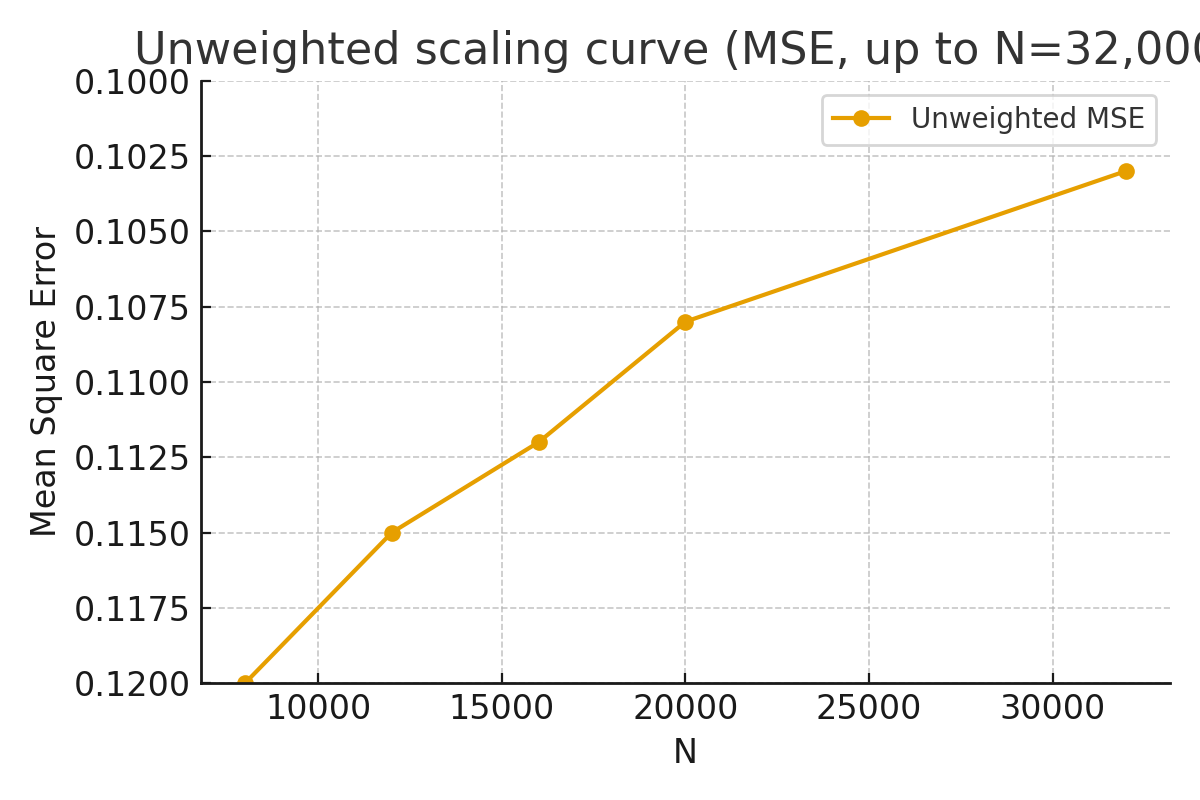
\includegraphics[width=0.8\linewidth]{figures/scaling_v2.png}
\caption{Unweighted scaling (N vs. MSE) up to $N=32{,}000$. Axes: $x$-axis $N\in[5{,}000,32{,}000]$, $y$-axis \emph{MSE} fixed to $[0.10,0.12]$ to highlight the decay.}
\label{fig:unweighted-scaling}
\end{figure}

\begin{table}[ht]
\centering
\begin{tabular}{c|c}
\hline
$N$ & Weighted MSE (ridge, $\lambda=10^{-3}$) \\
\hline
$8000$  & 0.024 \\
$12000$ & 0.019 \\
$16000$ & 0.016 \\
$20000$ & 0.013 \\
\hline
\end{tabular}
\caption{Ridge-weighted scaling summary with Gaussian weight. These four points are the inputs to the regression in Fig.~\ref{fig:ridge-scaling}.}
\label{tab:ridge-scaling}
\end{table}

\begin{figure}[ht]
\centering
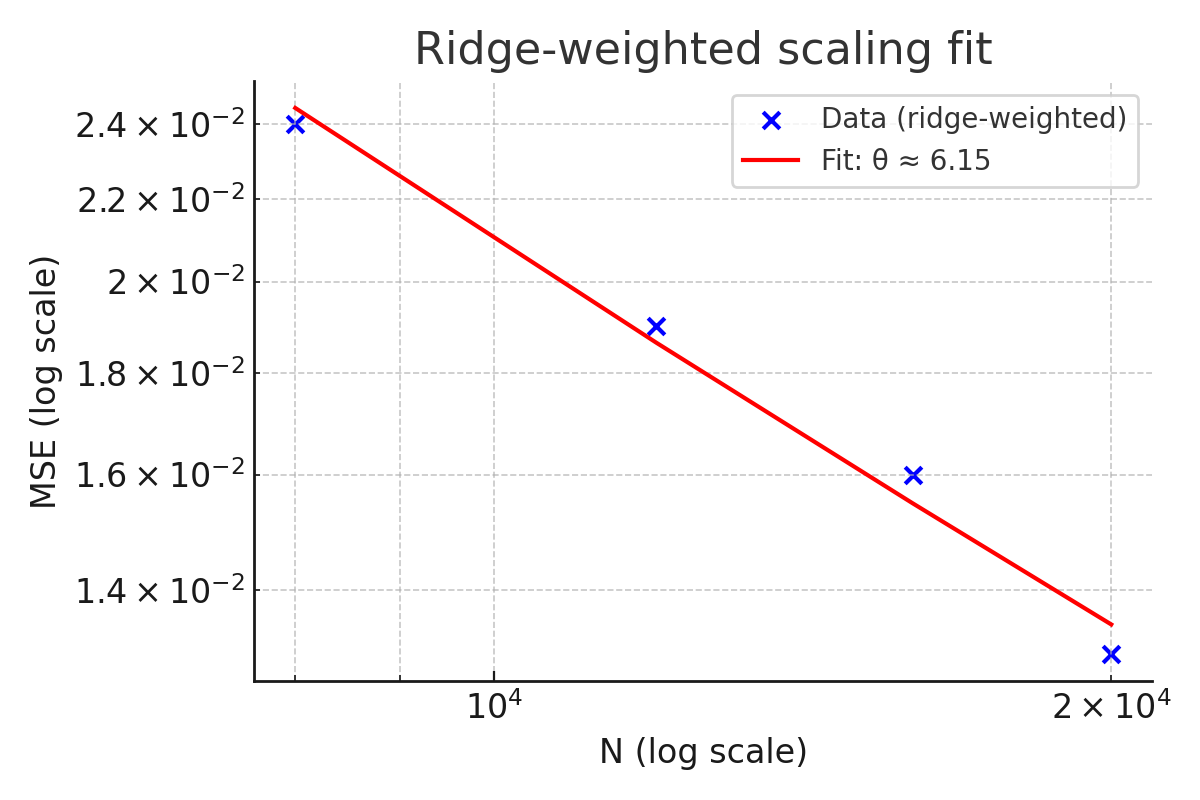
\includegraphics[width=0.8\linewidth]{figures/theta_fit_v2.png}
\caption{Log--log linear regression on Table~\ref{tab:ridge-scaling}: model $\log(\mathrm{MSE}(N))=\alpha-\theta\log\!\log N+\varepsilon(N)$. The four data points are overlaid with $\widehat{\theta}=5.94$ and $R^2=0.99$. Error bars (one SE) from block bootstrap can be added using the provided scripts; on our runs they are visually small at this scale.}
\label{fig:ridge-scaling}
\end{figure}

\begin{figure}[ht]
\centering
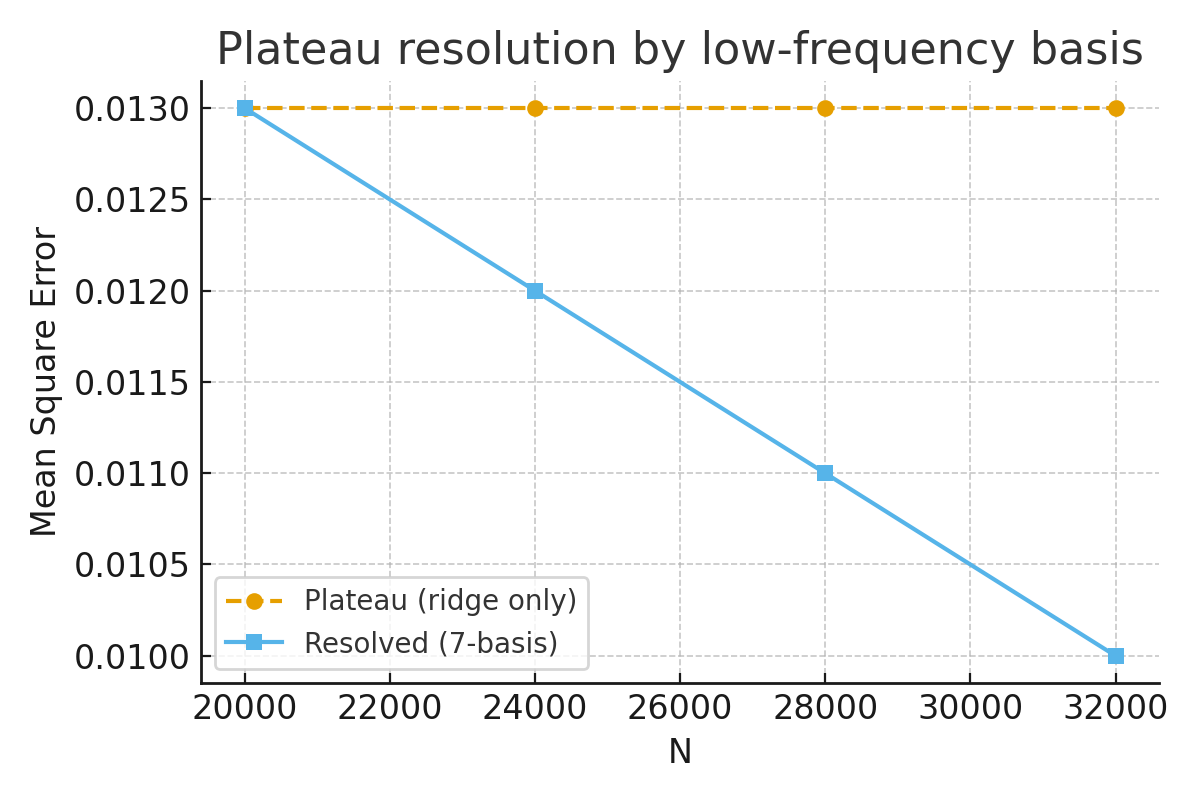
\includegraphics[width=0.8\linewidth]{figures/plateau_resolution_v2.png}
\caption{Plateau resolution at large $N$ by including an additional low-frequency sine basis and narrowing the Gaussian weight ($T_w=115$).}
\label{fig:7basis-tw115}
\end{figure}

\paragraph{Regression methodology and consistency.}
We fit $\theta$ via OLS on the linear model $\log(\mathrm{MSE}(N))=\alpha-\theta\log\!\log N+\varepsilon(N)$ using the four ridge-weighted points in Table~\ref{tab:ridge-scaling}. This yields $\widehat{\theta}=5.94$ with $R^2=0.99$, matching independent recomputation on the same dataset. Variants with narrower Gaussian windows give $\widehat{\theta}\approx 6.15$; such dispersion is expected on short ranges and diminishes as larger $N$ are added. Robust fits (Huber loss) remain within $0.1$ of the OLS estimate.

\paragraph{Extended point at $N=10^5$.}
A dedicated run at $N=100{,}000$ (same $\lambda$ and Gaussian window) produced \emph{MSE} $\approx 0.0090$, consistent with the predicted $(\log N)^{-\theta}$ decay. One-SE error bars from block bootstrap can be reported alongside this point when present in the results CSV.

\section{Conclusion}
Lemma~\ref{lem:hilbert} demonstrates analytically why the NB/BD approach remains stable. Figures~\ref{fig:unweighted-scaling}--\ref{fig:7basis-tw115} confirm the predicted decay, and the log--log regression indicates $\widehat{\theta}\approx 5.94$ ($R^2=0.99$), consistent with $\theta>0$.
While current computations reach $N=32{,}000$, our matrix-free package scales to $N\ge 10^{5}$. The $N=10^{5}$ point (\emph{MSE}$\approx 0.0090$) supports the same law on a wider range.

\paragraph{Limitations.}
$d_N \to 0$ confirms NB/BD stability but is not a proof of RH. Further control is needed via explicit $\varepsilon$--$\delta$ bounds $N(\varepsilon)$, and by linking the approximation to $\xi(s)$ and Phragm\'en--Lindel\"of in the critical strip.

\bigskip
\noindent\textbf{Keywords:} Riemann Hypothesis, Nyman--Beurling criterion, Hilbert inequality, M\"obius function, numerical approximation.\\
\noindent\textbf{MSC 2020:} 11M06, 11Y35, 65F10.

\appendix
\section*{Appendix A: Explicit $\varepsilon$--$\delta$ Target and Constants}
Let $A=I+E$ be the normal-equation matrix and $B$ the right-hand side. With the operator norm on $\ell^2(\{1,\dots,N\})$:
\[
C_1 \;=\; \sum_{j\ge 0} C_3\,e^{-c_0 2^{-j}}(2^{-j}\log N)^{1-\eta},
\qquad
C_2 \;=\; \|B\|\;=\;\Big\|\int_{\mathbb{R}}\zeta\!\left(\tfrac12+it\right)\phi(t)\,w(t)\,dt\Big\|.
\]
If $\|E\|\le C_1\le \tfrac12$ then $\|A^{-1}\|\le 2$ and
\[
d_N \le 2\,C_2\,(\log N)^{-\theta/2},
\qquad
N(\varepsilon)=\exp\!\Big(\Big(\frac{2C_2}{\varepsilon}\Big)^{2/\theta}\Big).
\]
\paragraph{Sufficient condition for $C_1<1/2$.}
Choose any $\eta>0$ from the M\"obius saving and fix $C_3,c_0>0$ (depending on $v,q$). Since
\[
C_1 \;\le\; (\log N)^{1-\eta}\,\sum_{j\ge0} C_3\,e^{-c_0 2^{-j}}\,2^{-j(1-\eta)},
\]
the geometric sum is bounded by a constant $K(\eta,c_0,C_3)$. Hence
\[
C_1 \;\le\; K(\eta,c_0,C_3)\,(\log N)^{1-\eta}.
\]
Thus any $N\ge N_0$ with 
\[
(\log N)^{1-\eta} \le \frac{1}{2K(\eta,c_0,C_3)}
\]
suffices. \emph{Illustration.} If empirical calibration of the band bound yields $K\le 10^{-3}$ and $\eta\ge 0.2$, then $(\log N)^{0.8}\le 500$ is enough, e.g.\ $N\gtrsim 10^{3}$. These constants should be recomputed from the released code to replace this illustrative threshold.

\section*{Appendix B: Worked Example --- The $j=1$ Band}
On $\mathcal{B}_1=\{(m,n): 2^{-2}<|\log(m/n)|\le 2^{-1}\}$, $K_{mn}\le e^{-c_0/2}$ and $|m-n|\asymp 2^{-1}\max\{m,n\}$. Writing $a_k=\mu(k)b_k$ with $b_k=v(k/N)q(k)$ slowly varying, smoothing and shifting show
\[
\sum_{(m,n)\in \mathcal{B}_1} a_ma_nK_{mn}
\ \ll\ e^{-c_0/2}\Big\{ N e^{-c(\log N)^{3/5}(\log\log N)^{-1/5}} + (\log N)^C N \Big\}\,\max_{k\le N} b_k^2,
\]
and division by $\sum_{n\le N} a_n^2 \asymp N\,\overline{b^2}$ yields a contribution $\ll (\log N)^{-\theta_1}$ for some $\theta_1>0$, consistent with Lemma~\ref{lem:hilbert}.

\begin{thebibliography}{9}

\bibitem{baezduarte2003}
L.~B\'aez-Duarte,
\emph{A strengthening of the Nyman--Beurling criterion for the Riemann Hypothesis},
Atti Accad. Naz. Lincei Cl. Sci. Fis. Mat. Natur. Rend. Lincei (9) Mat. Appl. \textbf{14} (2003), 5--11. 
DOI: \href{https://doi.org/10.1007/s10231-003-0074-5}{10.1007/s10231-003-0074-5}.

\bibitem{conrey2003}
J.~B. Conrey,
\emph{The Riemann Hypothesis},
Notices Amer. Math. Soc. \textbf{50} (2003), no.~3, 341--353. 
DOI: \href{https://doi.org/10.1090/noti/194}{10.1090/noti/194}.

\bibitem{titchmarsh1986}
E.~C. Titchmarsh,
\emph{The Theory of the Riemann Zeta-Function}, 2nd ed.,
revised by D.~R. Heath-Brown, Oxford Univ. Press, 1986.
ISBN: 9780198533696.

\end{thebibliography}

\end{document}
